\chapter{Introduction}
\section{Context}
Electromyography (EMG) is the technique of measuring the electrical activity that forms in a muscle in response to a nerve stimulating the muscle fibers \cite{biomechanics_research_methods} \cite{wikipedia_emg}. EMG is a popular method of measuring a person's intent to contract a muscle as it measures the muscle activation rather than the muscle contraction \cite{control_interfaces_intention_detection}\cite{human_robotics}. This means that it can still be used in scenarios where muscles can not respond accurately to nerve stimulation due to for example muscular dystrophy \cite{emg_arm_function_boys_pilot}. As a result, EMG is a good way of creating a control interface for exo-aids in various scenarios. Additionally, the amplitude of the EMG signal has a roughly linear relation with the force produced by the muscles and is therefore suitable for human machine interfaces \cite{adaptive_filter_dry_electrode}.

The electrical activity of a muscle can either be measured by probing the inside of a muscle (called intramuscular EMG or iEMG), or by measuring the electrical potential on the surface of the skin (called surface EMG or sEMG). iEMG has a high selectivity for individual motor neuron units which is desirable for a precise control interface registering multiple degree of freedoms \cite{semg_vs_iemg}, but has as a downside that it is an invasive and difficult procedure \cite{intramuscular_emg_signals}. sEMG is a non-invasive method of measuring requiring only sticking electrodes on the skin but this method can only measure the combined electrical activity of many muscle fibers resulting in a noisy and imprecise signal \cite{wiki:Electromyography}. 

During the last two decades research has attempted to gather more accurate sEMG readings by increasing the number of electrodes on a muscle with a technique called high-density sEMG \cite{high_density_semg}. 
This technique has allowed the measuring of spatial muscle activation in addition to time domain muscle activation. By measuring the muscle activation of a single muscle at multiple points in space it is theoretically possible to determine the behaviour of individual motor units \cite{high_density_semg_clinical_applications}.

However, this increased accuracy comes with a catch: each electrode outputs a single data stream that needs to be processed. Adding more electrodes means requiring more amplifier channels and smaller electrodes with higher contact impedance \cite{electrode_size_impedance}, both of which results in more expensive amplifiers. Additionally, having to process more data requires a faster signal processing chain that should retain the original processing quality.

This project aims to give an overview of the effectiveness of various EMG processing techniques. The effect of whitening the input signal, different filtering techniques, and different envelope detection techniques are discussed, with the overarching goal of performing accurate force estimation from sEMG signals.

\section{Related work}
There are a number of works on applying different filtering techniques in the medical field. Some interesting papers that closely relate to this assignment are discussed.

An example that shows the effectiveness of adaptive filters for real-time signal processing is the work by M. Hanine et al. \cite{adaptive_filter_emg_noise_cancellation_ecg} which covers the removal of an EMG signal from an electrocardiogram (ECG, electrical activity around the heart) signal. This is notable because the signal spectra of EMG and ECG overlap to a large extend and are therefore notoriously hard to remove using static filters. Furthermore it is mentioned in \cite{influence_semg_amplitude_estimation_technique_on_emg_force_relationship} that adaptive filters might be the most suitable type of filters for estimating force from sEMG signals.

The performance of adaptive filters and Wiener filters for noise cancellation in real-time environments in general has been tested in \cite{wiener_vs_adaptive_realtime_noisecancellation}. This report provides a solid groundwork for an intuitive understanding of wiener filters and adaptive filters which are used in this project.

A bold but promising implementation of Wiener filter in sEMG is presented in the work of J. Liu et al \cite{wiener_filter_a_priori_semg}. This paper presents the problem of voluntary EMG signals being contaminated by spontaneous unwanted motor activity from paretic muscles in for example stroke or spinal cord injury patients. The research uses an 'a priori' SNR (deduced from theory, not measurements) to filter the EMG signal from the involuntary muscle contractions. 

A common technique of improving signal to noise ratio (SNR) through pre-processing is 'whitening'. Whitening decorrelates the sEMG signal to yield improved signal accuracy \cite{emg_whitening}. 
Whitening can primarily be used for high-amplitude EMG signals and has trouble retaining effectiveness on low amplitude signals. This problem has been attempted to solve by creating adaptive whitening filter which shows promising results when applied to low EMG amplitude signals \cite{adaptive_whitening}. 

An important paper in the field of EMG signals is \cite{optimal_myoprocessor}. This research aims to provide a fully mathematical solution for an optimal myoelectric signal processor, and to do so a phenomenological mathematical model of myoelectric activity is presented. In other words: This paper uses biology, physics and statistics to create a framework that predicts the EMG signal from muscle activity.

There are several papers related to signal processing of sEMG signals.
One outstanding example is the work by M.Z. Jamal et al \cite{adaptive_filter_dry_electrode} from 2019, where it is shown that adaptive filters are an effective solution to EMG signal processing. The paper presents the instrumentation scheme of a dry-electrode sEMG measurement setup and explains a method of creating real-time adaptive finite impulse response (FIR) filters. In essence this is close to the aim of this research project, but this report is aimed at comparing the performance between filters rather than the creation of a specific one.


Lastly it should be mentioned that static and adaptive filters are only a subset of the available tools for sEMG signal processing. An emerging topic in this field is the use of machine learning methods for signal analysis. Applying machine learning could allow for fast, efficient, and effective signal processing, with the downside of unexpected behaviour in certain situations. Where static filters and adaptive filters exhibit deterministic behaviour (which is difficult to confirm in the case of real-time adaptive filters), machine learning methods can be somewhat 'hit or miss'. \cite{ml_semg_processing_1,ml_semg_processing_2}. It has been found that machine learning models at times violate their original expectations after deployment. The main reason for this is that the models often contain varying and unknown failure modes that are only revealed after deployment due to the complexity of the model and the lack of understanding of internal systems (black-box behaviour) \cite{microsoft_machine_learning_reliable}.

\section{Research goal}
Even though a significant amount of research has been done into the digital processing of sEMG signals, an overview comparing different techniques is lacking. This report aims to give an overview of pre-whitening, different filtering techniques, and multiple envelope detection techniques. The goal of this project is to explore the difference in performance of different sEMG signal processing chains when applied to sEMG signals for real-time force estimation.
In Figure~\ref{fig:global_thesis_flowchart} a high-level overview of the signal processing chain is presented. 

\begin{figure}[h!t]
	\begin{center}
		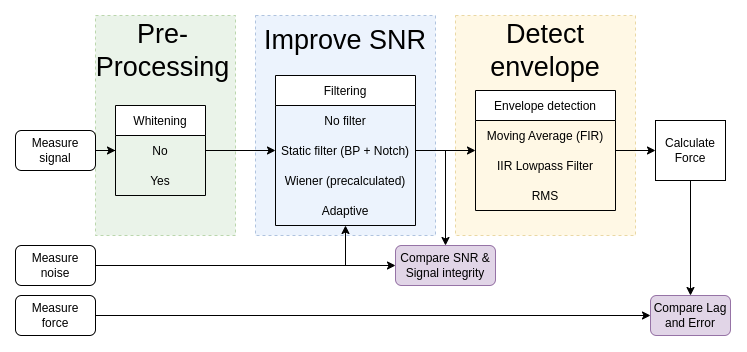
\includegraphics[width=1.0\columnwidth]{images/global_thesis_flowchart.png}
	\end{center}
	\caption{High-level overview of the signal processing chain}
	\label{fig:global_thesis_flowchart}
\end{figure}

These research efforts are driven by the research question below.

\begin{quote}\emph{What is the best combination of whitening, filtering, and envelope detection to estimate force from sEMG in real-time? }\end{quote}

This report consists of three main sections:
\begin{itemize}
    \item In the theory section the background of each option in each processing step (whitening, filtering, and envelope detection) is explained
    \item In the simulation section it is shown how different parameters influence the behaviour of each option in a simulated environment
    \item In the measurements section it is shown how all possible combinations from each processing step perform on a measured sEMG signal to find the optimal sEMG processing chain
\end{itemize}

\cmgk{Finish each chapter with a short conclusion. About a quarter page is mostly sufficient.}
